\chapter{Experimental tests}
This chapter will be concerned with

\section{Ideal experimental conditions}
In this brief section we will present what the ideal experiment to verify quantum mechanics against local-realism would be within the argument presented in chapter \ref{chap:ghz-theorem}.%rephrasing might be needed. why ideal?

We have noticed in \S \ref{sec:adaptation-to-3-particles} that the state (\ref{eq:ghz-state}) is an eigenstate of all observables (\ref{eq:xyy-observables}) and (\ref{eq:xxx-observable}), moreover it is easy to prove that all these observables commute with each other. This implies that, in principle, we could verify the quantum mechanical predictions with a single apparatus that measures subsequently the observables (\ref{eq:xyy-observables}) and (\ref{eq:xxx-observable}). In addition, a single run of the experiment would suffice to verify such predictions.

Realizing this experiment would involve putting three particles in state (\ref{eq:ghz-state}) and designing apparatuses that measure the product of three spin components.

To our knowledge no attempt on this approach has been made. 

\begin{observation}
SINGLE PRODUCT VS SUBSEQUENT MEASUREMENTS OF PRODUCTS
\end{observation}

\section{Actual experiments}
In this section we will present an experimental approach that has actually been pursued to verify the quantum mechanical predictions against local-realism.

\subsection{Observation of GHZ entanglement}

\begin{figure}
  \centering
  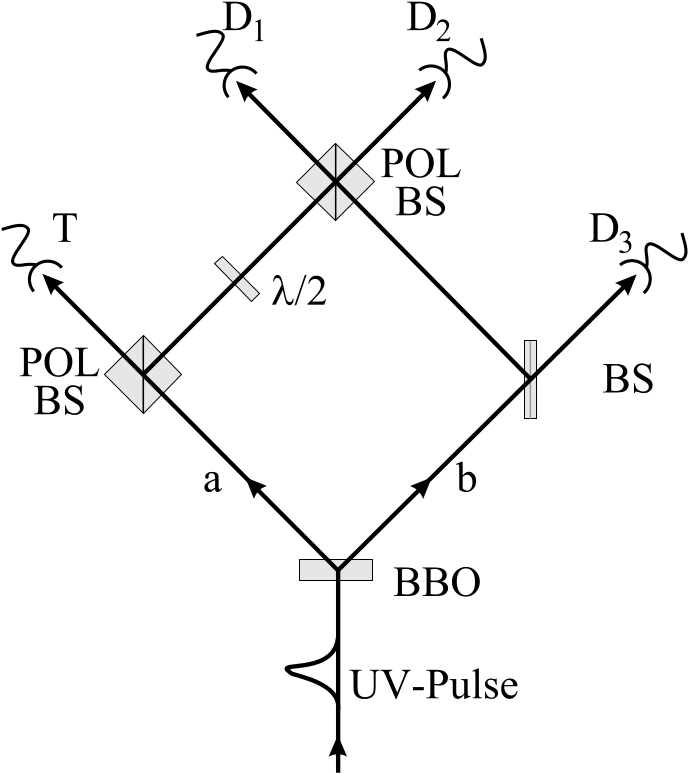
\includegraphics[width=0.5\textwidth]{Mainmatter/Chapter3/ghz-entanglement.png}
  \caption{HERE GOES THE CAPTION}
  \label{fig:ghz-entanglement}
\end{figure}

We begin this section by exposing a method that can be used to obtain systems of three particles exhibiting GHZ entanglement \cite{PhysRevLett.82.1345}.

Consider the experimental apparatus schematized in Fig. \ref{fig:ghz-entanglement}. Short pulses of ultraviolet light, which passes through a nonlinear crystal (BBO), generate pairs of polarization entangled photons in the state:
\begin{equation}
  \frac{1}{\sqrt{2}} \left( |H\rangle_a |V\rangle_b - |V\rangle_a |H\rangle_b \right),
\end{equation}
where the state $|H\rangle_a |V\rangle_b$ indicates a horizontally polarized photon in arm $a$ and a vertically polarized photon in arm $b$, conversely, the state $|V\rangle_a |H\rangle_b$ indicates a vertically polarized photon in arm $a$ and a horizontally polarized photon in arm $b$.

Continuing along arm $a$ we find a polarizing beam splitter that reflects vertically polarized photons and transmits horizontally polarized photons towards detector $T$. Reflected (vertically polarized) photons go then through a $\lambda/2$ plate that rotates polarization to $45^\circ$, then to a second polarizing beam splitter (analogous to the one already encountered) and finally to detectors $D_1$ ($V$ polarized photons) and $D_2$ ($H$ polarized photons).

Along arm $b$ we find a $50/50$ (polarization independent) beam splitter; transmitted photons go to detector $D_3$ while reflected photons go the second polarizing beam splitter of arm $a$ and finally to detectors $D_1$ ($H$ photons) and $D_2$ ($V$ photons).

All detectors, are behind narrow interference filters, the reason of which will be clarified later.

We want to show here that if two pairs are generated by a single pulse and each of the four photons is detected by one of the detectors $T$, $D_1$, $D_2$ and $D_3$ (exactly one photon per detector) then a three photon GHZ state is recorded by detectors $D_1$, $D_2$ and $D_3$.% a littel cumbersome, you want to reword it?

\subsection{Claims regarding local-realism}
